\documentclass[12pt,twoside]{report}

%%%%%%%%%%%%%%%%%%%%%%%%%%%%%%%%%%%%%%%%%%%%%%%%%%%%%%%%%%%%%%%%%%%%%%%%%%%%%

% Definitions for the title page
% Edit these to provide the correct information

\newcommand{\reporttitle}{Análisis de componentes principales}
\newcommand{\reportauthor}{David Alberto Martín Vela}
\newcommand{\subject}{Estadística multivariante}
\newcommand{\degreetype}{Doble Grado Ingeniería Informática y Matemáticas}
\newcommand{\email}{\href{mailto:davidmv1996@correo.ugr.es}{davidmv1996@correo.ugr.es}}

%%%%%%%%%%%%%%%%%%%%%%%%%%%%%%%%%%%%%%%%%%%%%%%%%%%%%%%%%%%%%%%%%%%%%%%%%%%%%

% load some definitions and default packages
%%%%%%%%%%%%%%%%%%%%%%%%%%%%%%%%%%%%%%%%%
% University Assignment Title Page 
% LaTeX Template
% Version 1.0 (27/12/12)
%
% This template has been downloaded from:
% http://www.LaTeXTemplates.com
%
% Original author:
% WikiBooks (http://en.wikibooks.org/wiki/LaTeX/Title_Creation)
%
% License:
% CC BY-NC-SA 3.0 (http://creativecommons.org/licenses/by-nc-sa/3.0/)
% 
%
%%%%%%%%%%%%%%%%%%%%%%%%%%%%%%%%%%%%%%%%%
%----------------------------------------------------------------------------------------
%	PACKAGES AND OTHER DOCUMENT CONFIGURATIONS
%----------------------------------------------------------------------------------------
\usepackage[a4paper,hmargin=2.8cm,vmargin=2.0cm,includeheadfoot]{geometry}
\usepackage{textpos}
\usepackage{tabularx,longtable,multirow,subfigure,caption}%hangcaption
\usepackage{fncylab} %formatting of labels
\usepackage{fancyhdr} % page layout
\usepackage{url} % URLs
\usepackage[english]{babel}
\usepackage{amsmath}
\usepackage{graphicx}
\usepackage{dsfont}
\usepackage{epstopdf} % automatically replace .eps with .pdf in graphics
\usepackage{array}
\usepackage{latexsym}
\usepackage{booktabs}
\usepackage[pdftex,hypertexnames=false,colorlinks]{hyperref} % provide links in pdf
\usepackage[
    type={CC},
    modifier={by-nc-sa},
    version={3.0},
]{doclicense}
\usepackage[
backend=bibtex,
style=alphabetic,
sorting=ynt
]{biblatex}
\addbibresource{refs.bib}

\usepackage{listings}
\usepackage{color}
\usepackage{multicol}
\definecolor{dkgreen}{rgb}{0,0.6,0}
\definecolor{gray}{rgb}{0.5,0.5,0.5}
\definecolor{mauve}{rgb}{0.58,0,0.82}

\lstset{frame=tb,
  language=R,
  aboveskip=0.5mm,
  belowskip=0.5mm,
  showstringspaces=false,
  columns=flexible,
  basicstyle={\small\ttfamily},
  numbers=none,
  numberstyle=\tiny\color{gray},
  keywordstyle=\color{blue},
  commentstyle=\color{dkgreen},
  stringstyle=\color{mauve},
  breaklines=true,
  breakatwhitespace=true,
  tabsize=1
}

\hypersetup{pdftitle={},
  pdfsubject={}, 
  pdfauthor={},
  pdfkeywords={}, 
  pdfstartview=FitH,
  pdfpagemode={UseOutlines},% None, FullScreen, UseOutlines
  bookmarksnumbered=true, bookmarksopen=true, colorlinks,
    citecolor=black,%
    filecolor=black,%
    linkcolor=black,%
    urlcolor=black}

\usepackage[all]{hypcap}


%\usepackage{color}
%\usepackage[tight,ugly]{units}
\usepackage{float}
%\usepackage{tcolorbox}
%\usepackage[colorinlistoftodos]{todonotes}
% \usepackage{ntheorem}
% \theoremstyle{break}
% \newtheorem{lemma}{Lemma}
% \newtheorem{theorem}{Theorem}
% \newtheorem{remark}{Remark}
% \newtheorem{definition}{Definition}
% \newtheorem{proof}{Proof}


%%% Default fonts
\renewcommand*{\rmdefault}{bch}
\renewcommand*{\ttdefault}{cmtt}
\renewcommand{\contentsname}{Índice}

%%% Default settings (page layout)
\setlength{\parindent}{0em}  % indentation of paragraph

\setlength{\headheight}{14.5pt}
\pagestyle{fancy}
\renewcommand{\chaptermark}[1]{\markboth{\chaptername\ \thechapter.\ #1}{}} 

\fancyfoot[ER,OL]{\sffamily\textbf{\thepage}}%Page no. in the left on odd pages and on right on even pages
\fancyfoot[OC,EC]{\sffamily }
\renewcommand{\headrulewidth}{0.1pt}
\renewcommand{\footrulewidth}{0.1pt}
\captionsetup{margin=10pt,font=small,labelfont=bf}


%--- chapter heading

\def\@makechapterhead#1{%
  \vspace*{10\p@}%
  {\parindent \z@ \raggedright \sffamily
    \interlinepenalty\@M
    \Huge\bfseries \thechapter \space\space #1\par\nobreak
    \vskip 30\p@
  }}

%---chapter heading for \chapter*  
\def\@makeschapterhead#1{%
  \vspace*{10\p@}%
  {\parindent \z@ \raggedright
    \sffamily
    \interlinepenalty\@M
    \Huge \bfseries  #1\par\nobreak
    \vskip 30\p@
  }}

\allowdisplaybreaks

% load some macros
% Here, you can define your own macros. Some examples are given below.

\newcommand{\R}[0]{\mathds{R}} % real numbers
\newcommand{\Z}[0]{\mathds{Z}} % integers
\newcommand{\N}[0]{\mathds{N}} % natural numbers
\newcommand{\C}[0]{\mathds{C}} % complex numbers
\renewcommand{\vec}[1]{{\boldsymbol{{#1}}}} % vector
\newcommand{\mat}[1]{{\boldsymbol{{#1}}}} % matrix


\date{Curso 2020-2021}

\begin{document}

% load title page
% Last modification: 2015-08-17 (Marc Deisenroth)
\begin{titlepage}

\newcommand{\HRule}{\rule{\linewidth}{0.5mm}} % Defines a new command for the horizontal lines, change thickness here


%----------------------------------------------------------------------------------------
%	LOGO SECTION
%----------------------------------------------------------------------------------------


\includegraphics[width = 4cm]{../code/figures/ugr.png}\\[0.5cm] 

\center % Center remainder of the page

%----------------------------------------------------------------------------------------
%	HEADING SECTIONS
%----------------------------------------------------------------------------------------

\textsc{\Large Universidad de Granada}\\[0.5cm] 
\textsc{\large \subject}\\[0.5cm] 
\textsc{\today}\\[0.5cm] 

%----------------------------------------------------------------------------------------
%	TITLE SECTION
%----------------------------------------------------------------------------------------

\HRule \\[0.4cm]
{ \huge \bfseries \reporttitle}\\ % Title of your document
\HRule \\[1.5cm]
 
%----------------------------------------------------------------------------------------
%	AUTHOR SECTION
%----------------------------------------------------------------------------------------

\begin{minipage}{0.4\textwidth}
\begin{flushleft} \large
\reportauthor % Your name

\end{flushleft}
\end{minipage}
~


%----------------------------------------------------------------------------------------
%	FOOTER & DATE SECTION
%----------------------------------------------------------------------------------------
\vfill % Fill the rest of the page with whitespace
\email\\
\degreetype\\[0.5cm]

\makeatletter
\@date 
\makeatother


\end{titlepage}



% page numbering etc.
\pagenumbering{roman}
\clearpage{\pagestyle{empty}\cleardoublepage}
\setcounter{page}{1}
\pagestyle{fancy}



%%%%%%%%%%%%%%%%%%%%%%%%%%%%%%%%%%%%
%--- table of contents
\fancyhead[RE,LO]{\sffamily {Table of Contents}}
\begingroup
\pagestyle{plain}
\tableofcontents 
\endgroup

\clearpage{\pagestyle{empty}\cleardoublepage}
\pagenumbering{arabic}
\setcounter{page}{1}
\fancyhead[LE,RO]{\slshape \rightmark}
\fancyhead[LO,RE]{\slshape \leftmark}

%%%%%%%%%%%%%%%%%%%%%%%%%%%%%%%%%%%%
\chapter*{Introducción}
\addcontentsline{toc}{chapter}{Introducción}  

En este ejercicio práctico se pretende que el alumno emita un informe relacionado con la reducción de la dimensión mediante un análisis de componentes principales para alguno de los problemas planteados a continuación. Este informe debe incluir, como mínimo:

\begin{itemize}
	\item Un análisis exploratorio previo de los datos que incluya en distintos subapartados: un estudio descriptivo básico de cada variable para tener una visión de sus escalas y variabilidades; hay que tomar decisiones para el tratamiento de los posibles datos perdidos así como de los posibles valores extremos que aparezcan en algunas de las variables. En este análisis exploratorio, también, hay que justificar que los datos están correlados, tanto a nivel de muestra como a nivel poblacional con el test de Bartlett.
	\item El resultado obtenido para la reducción de la dimensión. Este apartado también puede incluir distintos subapartados que indiquen cuál es el número mínimo de componentes principales, así como su varianza explicada, que ilustren los pesos de cada variable en las componentes principales seleccionadas. Sería apropiado escribir de forma analítica estas componentes principales identificando cuáles de las variables originales correlacionan más con cada componente principal. Para esto último es de utilidad realizar e interpretar los distintos gráficos de correlaciones y biplot que incluyan las direcciones dos a dos o tres a tres, así como las observaciones con su aportación a la varianza explicada.
\end{itemize}


%%%%%%%%%%%%%%%%%%%%%%%%%%%%%%%%%%%%
\chapter*{Problema}
\addcontentsline{toc}{chapter}{Problema}  

He elegido el Problema 3 en el conjunto constituido por 34 estados del mundo se han observado 11 variables cuyos
resultados se recogen en el archivo estados.sav. Estas variables se han estandarizado,
pues están tomadas con unidades de medida muy diferentes. Estas variables son:
\begin{itemize}
\item Ztlibrop: Número de libros publicados.
\item Ztejerci: Cociente entre el número de individuos en ejército de tierra y población
total del estado.
\item Ztpobact: Cociente entre población activa y total.
\item Ztenergi: Tasa de consumo energético.
\item Zpservi: Población del sector servicios.
\item Zpagricu: Población del sector agrícola.
\item Ztmedico: Tasa de médicos por habitante.
\item Zespvida: Esperanza de vida.
\item Ztminfan: Tasa de mortalidad infantil.
\item Zpobdens: Densidad de población
\item Zpoburb: Porcentaje de población urbana
\end{itemize}

En este caso, se plantea la reducción del número de variables mediante un ACP. Se pide el informe con los datos estandarizados. Aunque la
variable Estado no se incluirá para la reducción de la dimensión, sí se pide, en la medida
de lo posible, que los distintos gráficos la incluyan para tener una visión más realista
desde un punto de vista comparativo entre estados. 

\chapter*{Análisis exploratorio}
\addcontentsline{toc}{chapter}{Análisis exploratorio}  

\section*{Carga de los datos y valores perdidos}
\addcontentsline{toc}{section}{Carga de los datos y valores perdidos}    

Cargamos los 34 estados del mundo sobre los que se han observado variables sociodemográficas y económicas:
\tiny \begin{verbatim}
> library(foreign)
> data <- read.spss("estados.sav", to.data.frame=TRUE)
> head(data, 34)
          PAIS     ZPOBDENS    ZTMINFAN    ZESPVIDA     ZPOBURB    ZTMEDICO     ZPAGRICU     ZPSERVI    ZTLIBROP    ZTEJERCI    ZTPOBACT    ZTENERGI
1     africasu -0.857191432  0.96148387 -1.54985484 -0.21488857 -0.73382516 -0.606355478  0.48366865 -0.57510397 -0.56042975 -0.78289704  0.12813846
2     argelia  -1.016717088  1.21338387 -0.89488793 -0.76526232 -0.88765979  0.057659570  0.05831739 -0.96961561 -0.20336698 -2.13409403 -0.52613591
3     argentin -0.991855947 -0.31857942  0.43886285  1.13811356  1.26602514 -0.759937190  0.78468647 -0.47636769 -0.48303442 -0.41890863 -0.37922198
4     australi -1.077834060 -1.02030085  1.08192126  1.28029344  0.49685195 -1.058066395  1.40635370  1.05949898 -0.61170369  0.62446672  1.18993245
5     brasil   -0.949384831  0.61190835 -0.32328046  0.44097348 -0.31077990  0.044108242  0.11066832 -0.53207948 -0.71491390 -0.42726448 -0.72526157
6     canada   -1.072654656 -1.02801208  1.12955522  0.81706220  0.51608128 -1.107754596  1.62884513  1.57708364 -0.86586064  0.96600967  2.74978482
7     chile    -0.945241307 -0.46766309  0.47458832  1.06473039 -0.79151315 -0.606355478  1.13151135 -0.69252676 -0.21044001 -0.71686695 -0.63345233
8     china    -0.022271439 -0.29287533  0.27214400 -1.71924349 -0.80112781  1.905157220 -1.88521069 -0.94691538 -0.38965874  1.70447158 -0.79477787
9     coreasur  2.861620943 -0.47280391  0.12924213 -0.04519000 -0.66652250  0.391925649 -0.50445505  0.77356425  1.16013447 -0.17435728 -0.51051973
10    egipto   -0.667625230  1.48070632 -1.02588131 -0.60473665 -1.13764108  0.712640400 -0.45864799 -0.88590734  0.24248176 -1.49621357 -0.82327121
11 espa\xf1a   -0.326820419 -1.01001922  1.07001277  0.68405522  0.97758519 -0.497944858  0.26117722  1.42826571  0.10236959 -0.54331956 -0.16396932
12    filipina  0.571288308  0.04641855 -0.54954175 -0.93954734 -1.10879709  0.988184059 -0.55680598 -0.93307433 -0.72408567 -0.43581567 -0.87196431
13    francia  -0.052311985 -1.03829371  1.10573824  0.70240101  0.68914524 -0.958689993  0.93519538  0.93292103 -0.02807325  0.37448801  0.55588195
14    humgria   0.094783101 -0.69899983  0.47458832 -0.20112923  1.46793310 -0.240469635 -0.58298144  1.79320160  0.09042840  0.98956169  0.34057118
15    india     1.072654656  1.63493081 -1.45458692 -1.58165005 -0.86843046  1.801263710 -1.57764901 -0.95544574 -0.73628387 -0.19176720 -0.92243683
16    indonesi -0.280205779  1.40359407 -1.54985484 -1.63668742 -1.14725575  1.232107954 -0.74657808 -0.96750778 -0.76279250 -0.33334671 -0.91277562
17    iran     -0.850976147  0.70958386 -0.58526722 -0.40293294 -1.07033843  0.292549247 -0.67459556 -0.76440102 -0.07440193 -1.35279974 -0.70865028
18    israel    0.035737891 -0.67072534  0.86756846  1.40871398  1.16987849 -1.071617722  1.35400278  0.99209789  4.42620176 -0.32337231 -0.19539657
19    italia    0.842689099 -0.92776616  1.07001277  0.39510900  1.55446508 -0.705731880  0.43786159 -0.32373737 -0.25507169 -0.01157335  0.09841816
20    japon     2.152042537 -1.10255392  1.24864011  0.83999444  0.02573337 -0.881899137  0.85666899  0.25235156 -0.74296346  0.94726825  0.31655099
21    libano    1.561590433 -0.06153860 -0.06129369  0.80788931 -0.27232124 -0.705731880  1.13151135 -0.16469295  0.34209564 -1.43851975 -0.65883307
22    marrueco -0.635512923  1.33162265 -1.01397283 -0.76067587 -1.10879709  0.708123290 -0.76620967          NA -0.11195898 -1.25205613 -0.87754597
23    mejico   -0.726670440  0.13895324 -0.07320218  0.39052255 -0.31077990 -0.186264325  0.83703740 -0.94225917 -0.78996888 -0.98929097 -0.40072379
24    nigeria  -0.194227666  1.73774714 -2.14527929 -1.41195148 -1.13764108  1.728989963 -1.36824531 -0.92401149 -0.69868856 -0.03897427 -0.94559840
25    pakistan  0.001553821  1.90482367 -1.96665196 -1.36608700 -0.95496245  1.114663116 -0.74657808 -0.96875479 -0.20915128 -1.20039046 -0.92516252
26    polonia   0.081316649 -0.74783758  0.65321565  0.01443382  0.92951186 -0.010097068 -0.63533236  0.07157343 -0.03681498  1.36222493  0.75427998
27    rdaleman  0.504991931 -0.98431514  0.78420903  0.83999444  1.27563980 -0.877382028 -0.16417404  0.44844158  0.04855887  1.65256659  1.56719986
28    reinouni  1.293297284 -0.98431514  0.98665335  1.50961584  0.01611870 -1.234233653  1.21658160  1.75837557 -0.48919984  0.85527941  0.69960067
29    rfaleman  1.461109987 -0.96889269  0.91520242  1.21608317  0.93912653 -1.098720377  0.60145823  2.40236043 -0.10795229  0.46019499  1.05982477
30    rumania  -0.128967170 -0.54220493  0.48649681 -0.44879742  0.48723728 -0.005579958 -0.96252564  0.05946495  0.02611529  1.08311493  0.59174918
31    turquia  -0.508099574  1.06944101 -0.45427384 -0.64601468 -0.56076119  1.390206775 -1.17847321 -0.76872234  0.68707865  0.32878726 -0.74078430
32    urss     -0.974245972 -0.59361309  0.28405249  0.23916977  2.37171159 -0.439222439  0.01251033 -0.03092794  1.17613398  1.30446522  0.95562005
33    usa      -0.845796742 -0.97146310  0.97474486  0.72533325  0.68914524 -1.148408578  1.30819572  0.19806196 -0.42313576  0.88671706  2.65959005
34    vietnam   0.589934164  0.65817570 -0.79962002 -1.76969441 -1.00303577  1.832883474 -1.74778951 -0.92521141  1.92835266  0.72221179 -0.95066101
\end{verbatim}

\normalsize Vemos que el PAIS españa, está mal codificado (espa\slash xf1a) esto nos traerá problemas cuando queramos representar gráficamente. Luego lo renombramos a algo más entendible como espania. Tenemos entonces 11 variables observadas en 34 Estados del mundo, eliminamos la primera columna del data.frame (PAIS) ya que no aporta nada al ACP, pero la guardámos como carácter.

\footnotesize
\begin{verbatim}
> data[11, "PAIS"] <- "espania"
> datos_pca<-data[,-1]
> row.names(datos_pca) = as.character(data$PAIS)
> # Para añadirlo de nuevo, 
> summary(datos_pca)
    ZPOBDENS          ZTMINFAN          ZESPVIDA          ZPOBURB           ZTMEDICO      
 Min.   :-1.0778   Min.   :-1.1026   Min.   :-2.1453   Min.   :-1.7697   Min.   :-1.1473  
 1st Qu.:-0.8497   1st Qu.:-0.9586   1st Qu.:-0.7460   1st Qu.:-0.7320   1st Qu.:-0.8829  
 Median :-0.1616   Median :-0.3931   Median : 0.2781   Median : 0.1268   Median :-0.2916  
 Mean   : 0.0000   Mean   : 0.0000   Mean   : 0.0000   Mean   : 0.0000   Mean   : 0.0000  
 3rd Qu.: 0.5547   3rd Qu.: 0.8985   3rd Qu.: 0.9033   3rd Qu.: 0.8148   3rd Qu.: 0.8694  
 Max.   : 2.8616   Max.   : 1.9048   Max.   : 1.2486   Max.   : 1.5096   Max.   : 2.3717  
                                                                                          
    ZPAGRICU          ZPSERVI            ZTLIBROP          ZTEJERCI           ZTPOBACT      
 Min.   :-1.2342   Min.   :-1.88521   Min.   :-0.9696   Min.   :-0.86586   Min.   :-2.1341  
 1st Qu.:-0.8480   1st Qu.:-0.72858   1st Qu.:-0.9240   1st Qu.:-0.59889   1st Qu.:-0.6735  
 Median :-0.2134   Median : 0.03541   Median :-0.3237   Median :-0.20626   Median :-0.1067  
 Mean   : 0.0000   Mean   : 0.00000   Mean   : 0.0000   Mean   : 0.00000   Mean   : 0.0000  
 3rd Qu.: 0.7115   3rd Qu.: 0.85176   3rd Qu.: 0.7736   3rd Qu.: 0.07996   3rd Qu.: 0.8789  
 Max.   : 1.9052   Max.   : 1.62885   Max.   : 2.4024   Max.   : 4.42620   Max.   : 1.7045  
                                      NA's   :1                                             
    ZTENERGI      
 Min.   :-0.9507  
 1st Qu.:-0.7813  
 Median :-0.3900  
 Mean   : 0.0000  
 3rd Qu.: 0.5828  
 Max.   : 2.7498  
\end{verbatim}
\normalsize

Como comentaba la descripción del problema, dado que las variables presentan unidades de medida muy diversas así como varianzas muy distintas, se han estandarizado previamente para evitar que algunas puedan anular o minimizar los efectos de otras. El análisis ACP se basará, por tanto, en dichas variables (ACP de matriz de correlaciones de variables sin estandarizar). Destacamos la variable \textbf{ZTLIBROP} con 1 valor perdido.
 
Para hacer un análsis exploratorio de los datos, auxiliarmente usaremos la librería DataExplorer de R \cite{data-explorer}. Hacemos un plot de los valores perdidos en la figura [\ref{fig:plot_missing}] una función que nos permite ver el porcentaje de valores perdidos de nuestra variable y número. También mostramos un histograma general de nuestros datos en la figura [\ref{fig:plot_hist}]. 

 \begin{lstlisting}
> library(DataExplorer)
> plot_missing(datos_pca)
> plot_histogram(datos_pca)
> plot(datos_pca)
\end{lstlisting}

\begin{figure}[H]
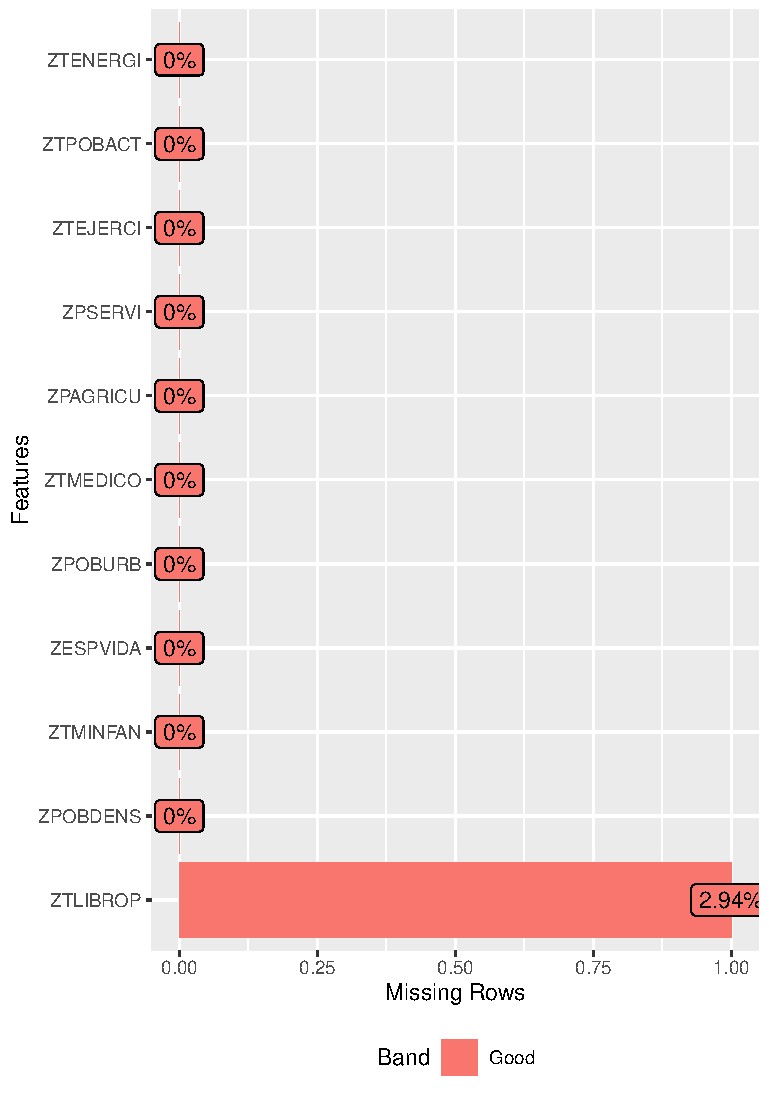
\includegraphics[width=\textwidth]{../code/figures/plot_missing.pdf}
\caption{plot\_missing}
\label{fig:plot_missing}
\end{figure} 

\begin{figure}[H]
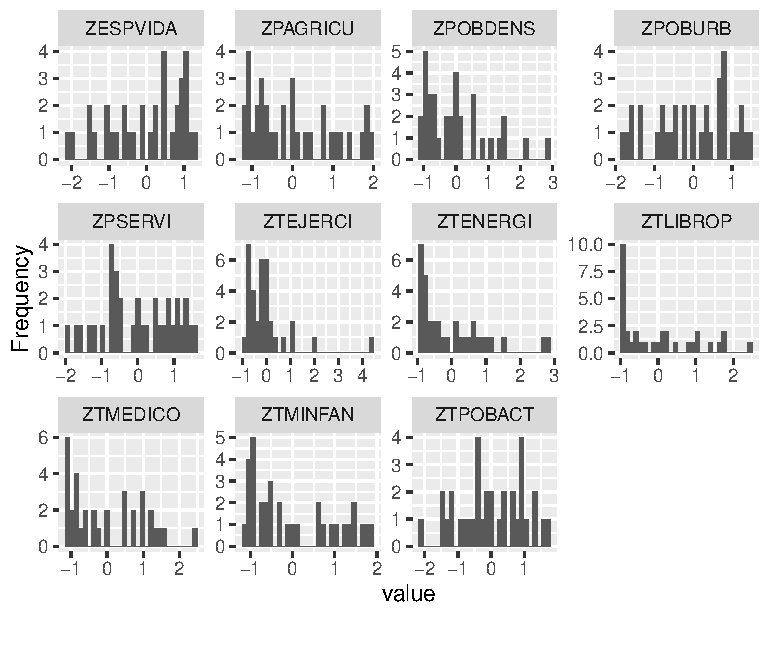
\includegraphics[width=\textwidth]{../code/figures/plot_histogram.pdf}
\caption{plot\_hist}
\label{fig:plot_hist}
\end{figure} 

\normalsize Para realizar la matriz de correlaciones y ver si tiene sentido un PCA, vamos a tratar con el valor perdido de la variable \textbf{ZTLIBROP} sustituyendolo por la media, ya que es únicamente 1 valor perdido.

\footnotesize \begin{verbatim}
> # For data frames, a convenient shortcut to compute the total missing values in
> # each column is to use colSums():
> colSums(is.na(datos_pca))
ZPOBDENS ZTMINFAN ZESPVIDA  ZPOBURB ZTMEDICO ZPAGRICU  ZPSERVI ZTLIBROP 
       0        0        0        0        0        0        0        1
ZTEJERCI ZTPOBACT ZTENERGI 
       0        0        0 
> # Se observa que en los datos hay algunos valores perdidos (NA). Hay que hacer 
> # un tratamiento detallado de estos valores perdidos. En este caso los vamos a
> # sustituir por la media.
> not_available<-function(data,na.rm=F){
+   data[is.na(data)]<-mean(data,na.rm=T)
+   data
+ }
> datos_pca$ZTLIBROP<-not_available(datos_pca$ZTLIBROP)
> colSums(is.na(datos_pca))
ZPOBDENS ZTMINFAN ZESPVIDA  ZPOBURB ZTMEDICO ZPAGRICU  ZPSERVI ZTLIBROP 
       0        0        0        0        0        0        0        0 
ZTEJERCI ZTPOBACT ZTENERGI 
       0        0        0 
\end{verbatim}
\normalsize

Observamos que no quedan valores nulos, luego no debemos preocuparnos de cómo imputarlos.
También podemos usar un boxplot para observar la distribución de cada variable con mayor comodidad, visualizamos la figura [\ref{fig:boxplot}]

 \begin{lstlisting}
> par(cex.axis=0.5) # is for x-axis
> boxplot(datos_pca,main="EDA",
+         ylab="z-values",
+         ylim=c(-3,5),
+         las=2,
+         col=c(1:11))
> 
\end{lstlisting}

\begin{figure}[H]
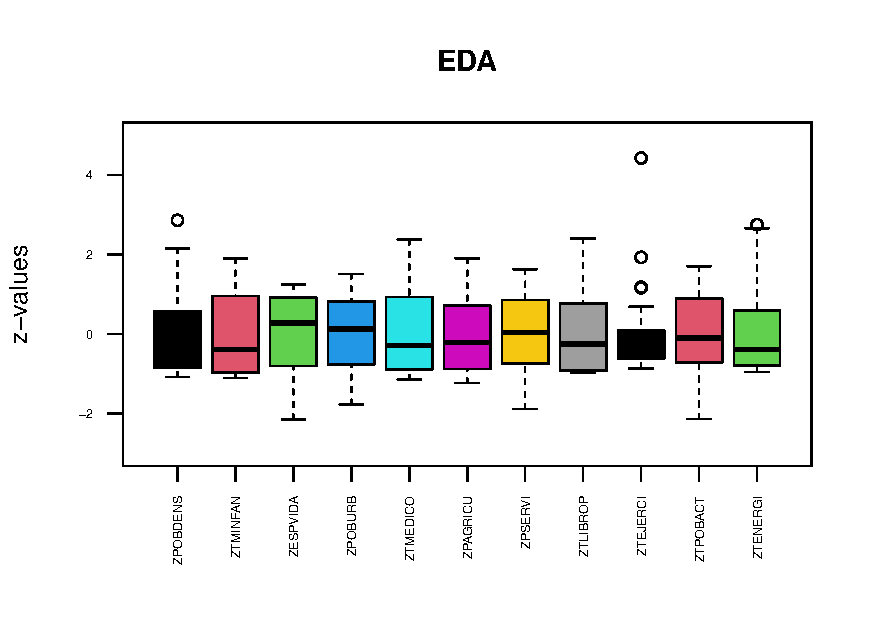
\includegraphics[width=\textwidth]{../code/figures/boxplot.pdf}
\caption{Boxplot de valores}
\label{fig:boxplot}
\end{figure} 

Vemos que nuestros valores tienen la misma escala pero presentan outliers en las variables \textbf{ZPOBDENS}, \textbf{ZTEJERCI} y  \textbf{ZTENERGI}. También algunas distribuciones son algo asimétricas teniendo la mediana aproximada al primer cuartil.

\section*{Análisis de la correlación de las variables}
\addcontentsline{toc}{section}{Análisis de la correlación de las variables}  

Vemos la matriz de correlaciones observadas entre las variables en la figura [\ref{fig:plot}]. La matriz de correlaciones observadas entre las variables, R, presenta en sus elementos fuera de la diagonal, lo que podríamos llamar información redundante o compartida por pares de variables originales.

\begin{figure}[H]
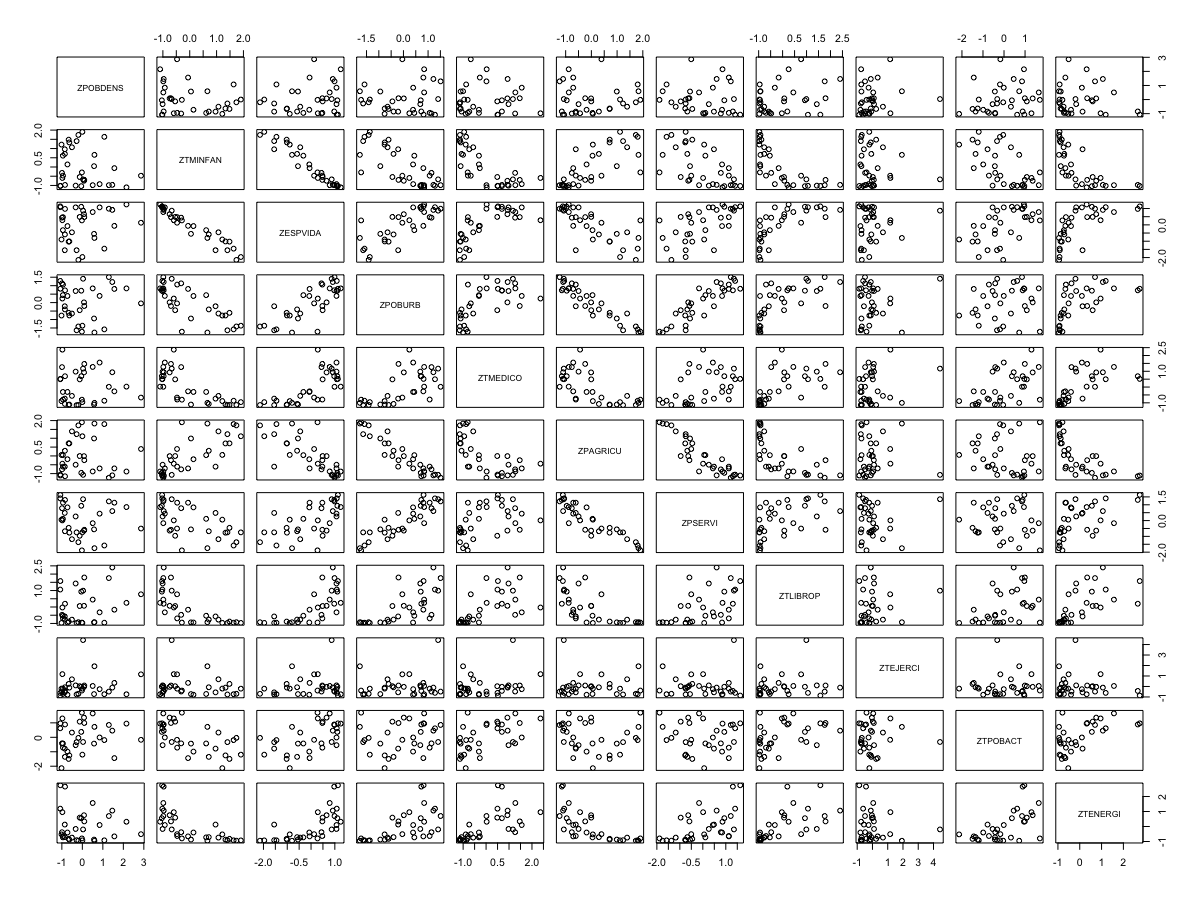
\includegraphics[width=\textwidth]{../code/figures/plot.png}
\caption{plot}
\label{fig:plot}
\end{figure} 

\begin{figure}[H]
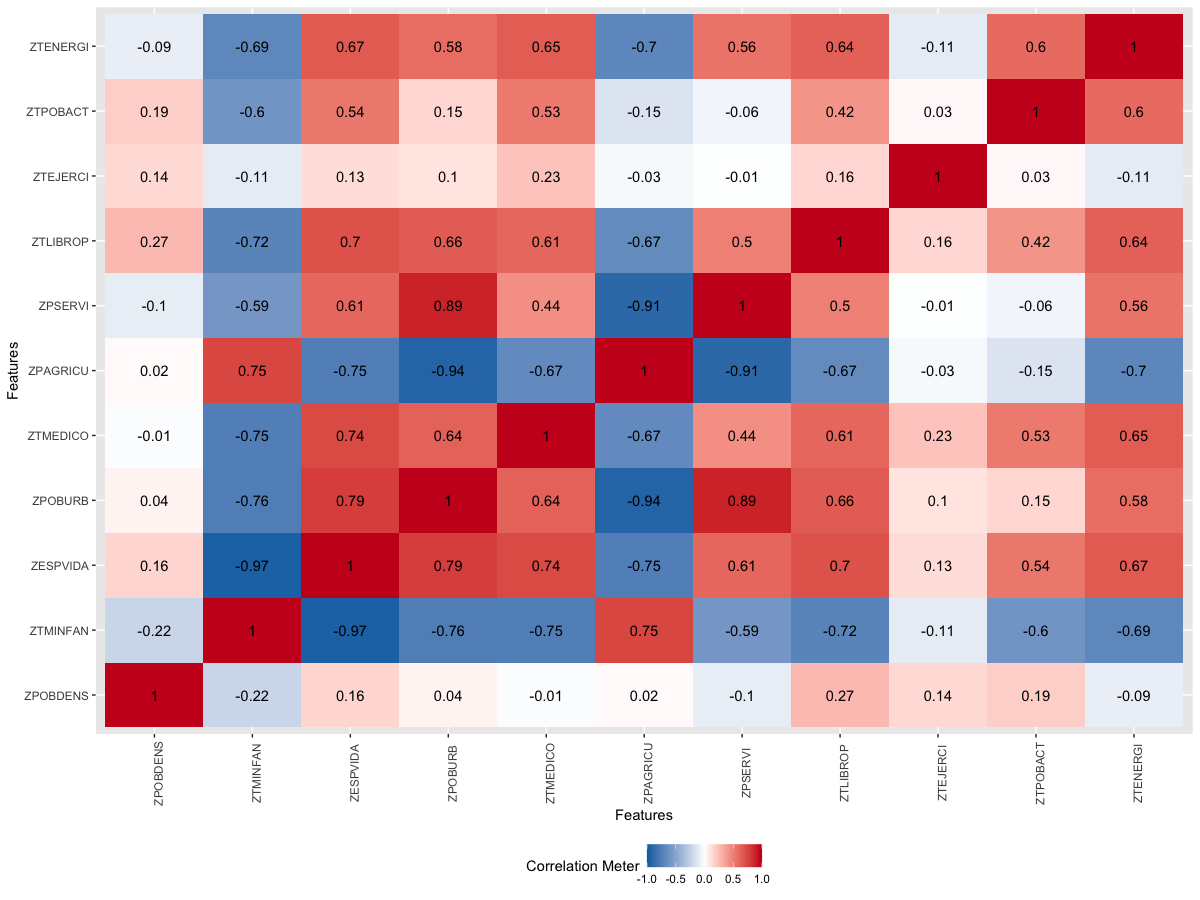
\includegraphics[width=\textwidth]{../code/figures/plot_corr.png}
\caption{plot}
\label{fig:corr_matrix}
\end{figure} 

Observando la matriz de datos existe correlación importante entre algunas variables
 \begin{lstlisting}
> cor(datos_pca$ZPSERVI,datos_pca$ZPOBURB)
[1] 0.8900152
> cor(datos_pca$ZESPVIDA,datos_pca$ZPOBURB)
[1] 0.787146
\end{lstlisting}

También vemos el determinante de la matriz de correlaciones, donde valores bajos son indicio de existencia de correlaciones entre las variables.

 \begin{lstlisting}
> det(cor(datos_pca ))
[1] 1.258756e-06
\end{lstlisting}

Por tanto, parece que podremos reducir en cierta medida el número de variables sin perder demasiada información. Nos aseguramos de esto realizando el Test de Bartlett, aplicado a los datos normalizados (que ya lo están).

 \begin{lstlisting}
> library(psych)
> # Se hace el test de esfericidad
> cortest.bartlett(cor(datos_pca), n = 34)
$chisq
[1] 387.1835

$p.value
[1] 1.865976e-51

$df
[1] 55
\end{lstlisting}

Observamos un \textbf{p-valor} prácticamente nulo, por lo que rechazamos la hipótesis nula y concluimos que los datos están correlados, por lo que procedemos con el Análisis de Componentes Principales.

\section*{Outliers}
\addcontentsline{toc}{section}{Outliers}  

El objetivo es el de localizar y tratar con outliers que puedan dar lugar a resultados erróneos ya que el ACP es muy sensible a valores extremos. Un diagrama de  cajas como el de la figura [\ref{fig:boxplot}] puede dar esta primera información. Vemos que nuestros valores tienen la misma escala pero presentan outliers en las variables \textbf{ZPOBDENS}, \textbf{ZTEJERCI} y  \textbf{ZTENERGI}. Sustituimos estos outliers por la media realizando justo el número necesario de pasadas en cada columna que presente outliers.

\begin{lstlisting}
> # Los outliers deben ser tratados de forma independiente por el investigador, 
> # de modo que para el ACP es necesario eliminarlos
> outlier<-function(data,na.rm=T){
+   H<-1.5*IQR(data)
+   data[data<quantile(data,0.25,na.rm = T)-H]<-NA
+   data[data>quantile(data,0.75, na.rm = T)+H]<-NA
+   continue<-any(is.na(data)) 
+   data[is.na(data)]<-mean(data,na.rm=T)
+   data[is.na(data)]<-mean(data,na.rm=T)
+   data
+ }
\end{lstlisting}

Y aplicamos esta función a las dos columnas que presentan outliers

\begin{lstlisting}
> datos_pca$ZPOBDENS<-outlier(datos_pca$ZPOBDENS)
> datos_pca$ZTEJERCI<-outlier(datos_pca$ZTEJERCI)
> datos_pca$ZTENERGI<-outlier(datos_pca$ZTENERGI)
\end{lstlisting}

En la figura [\ref{fig:boxplot_comparison}] comparamos los datos estandarizados antes y después de eliminar los outliers. Apreciamos que la estandarización ha centrado las distribuciones en el 0 y ha equiparado las escalas de las variables, pero se mantienen los outliers (comparar boxplot de la izquierda con figura [\ref{fig:boxplot}]). 

\begin{lstlisting}
> # Comparamos los datos originales y los arreglados 
> par(mfrow=c(1,2))
> # Boxplot de los datos originales
> boxplot(datos_originales,main="Datos originales",
+         ylab="z-values",
+         ylim=c(-3,5),
+         las=2,
+         col=c(1:11))
> # Boxplot de los datos corregidos.
> boxplot(datos_pca,main="Datos sin outliers",
+         ylab="z-values",
+         ylim=c(-3,5),
+         las=2,
+         col=c(1:11))
\end{lstlisting}

\begin{figure}[H]
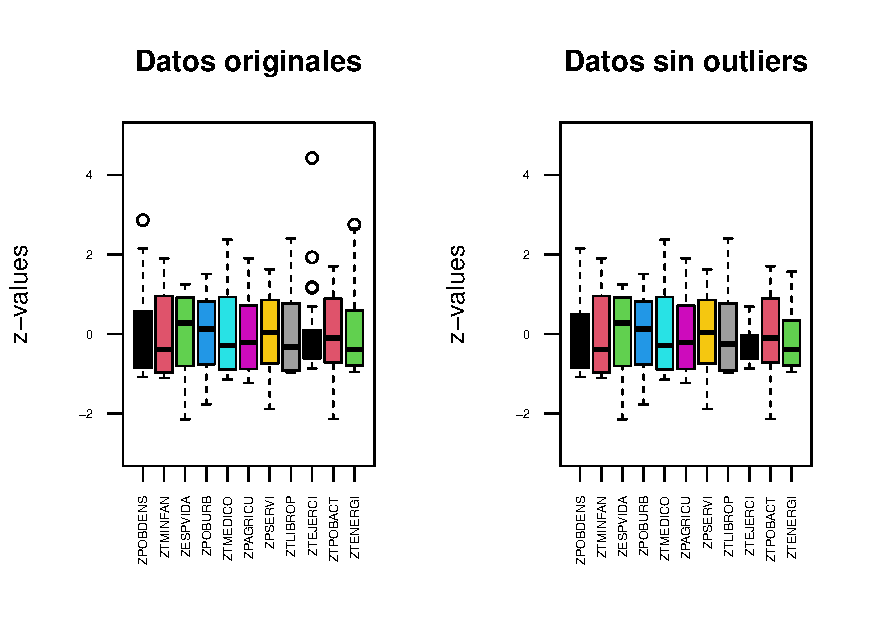
\includegraphics[width=\textwidth]{../code/figures/boxplot_comparison.pdf}
\caption{Limpieza de outliers}
\label{fig:boxplot_comparison}
\end{figure} 

\chapter*{Análisis de Componentes Principales}
\addcontentsline{toc}{chapter}{Análisis de Componentes Principales}  

\section*{Obtención componentes principales y varianzas}
\addcontentsline{toc}{section}{Obtención componentes principales y varianzas}  

Una vez visto que en este caso tiene sentido el PCA:

\begin{lstlisting}
> PCA<-prcomp(datos_pca, scale=T, center = T)
\end{lstlisting}

En el campo "rotation" del objeto "PCA" es una matrix cuyas columnas son los coeficientes de las componentes principales, es decir, el
peso de cada variable en la correspondiente componente principal. Los vectores propios de la matriz de correlaciones son las columnas de la matriz rotation.
Podemos consultar el peso de cada variable en cada componente principal:

\scriptsize \begin{verbatim}
> # Matriz de vectores propios
> PCA$rotation
                 PC1         PC2         PC3          PC4         PC5         PC6         PC7         PC8
ZPOBDENS  0.06796131  0.39036079  0.07578571 -0.873056137  0.05981546 -0.24337351  0.09619809 -0.04353317
ZTMINFAN -0.37529798 -0.11573027 -0.08212636 -0.014741875  0.41788865 -0.01756878  0.05245475 -0.39097670
ZESPVIDA  0.37165513  0.07270402 -0.00407411  0.012970861 -0.53281544  0.03028763 -0.04105430  0.29289664
ZPOBURB   0.35808785 -0.29124050 -0.06094609 -0.113795410 -0.05152603 -0.07065324 -0.10651593 -0.29868358
ZTMEDICO  0.33374417  0.13909259 -0.09587119  0.280930962  0.15782496 -0.36060911  0.78403566 -0.06560314
ZPAGRICU -0.36224935  0.29940891  0.04348437  0.061235615 -0.15998056  0.13248858  0.09343760 -0.01200167
ZPSERVI   0.29607632 -0.48878963  0.09183567 -0.148420697 -0.03064997 -0.07352269 -0.09280074 -0.37422057
ZTLIBROP  0.32594252  0.08892433 -0.07078859 -0.135187927  0.28062939  0.85707761  0.21913126 -0.01229527
ZTEJERCI  0.02397325  0.17948476 -0.93319975 -0.006241743 -0.12518016 -0.02870986 -0.16141551 -0.18218984
ZTPOBACT  0.20289865  0.56167354  0.29659750  0.281932179 -0.11796713  0.02948798 -0.25103160 -0.61023870
ZTENERGI  0.33155119  0.20152127 -0.02054058  0.148110844  0.61275026 -0.21278600 -0.45367225  0.34643517
                  PC9        PC10         PC11
ZPOBDENS  0.022846323 -0.01646372 -0.016686681
ZTMINFAN -0.157260993 -0.47091956 -0.511610948
ZESPVIDA -0.091799724 -0.54354628 -0.424556791
ZPOBURB  -0.792450091  0.16228759  0.088144761
ZTMEDICO  0.001929436 -0.06125296  0.058614024
ZPAGRICU -0.325592955 -0.48343682  0.617855535
ZPSERVI   0.449245272 -0.39418278  0.361609762
ZTLIBROP  0.015266047 -0.02755826  0.008370356
ZTEJERCI  0.127931321  0.01085377  0.063899183
ZTPOBACT  0.097328148  0.08409493 -0.095710436
ZTENERGI -0.066593066 -0.23535405  0.143880098
\end{verbatim}
\normalsize

También podemos ver los valores propios o varianzas de las componentes como una tabla o gráficamente en la figura [\ref{fig:varianza_total}]

\begin{lstlisting}
> summary(PCA)$sdev^2
 [1] 6.15934602 1.63988972 1.06319852 0.90543213 0.41577420 0.36326910 0.23219856 0.11250601 0.06208202 0.02696079
[11] 0.01934294
> screeplot(PCA)
\end{lstlisting}

\begin{figure}[H]
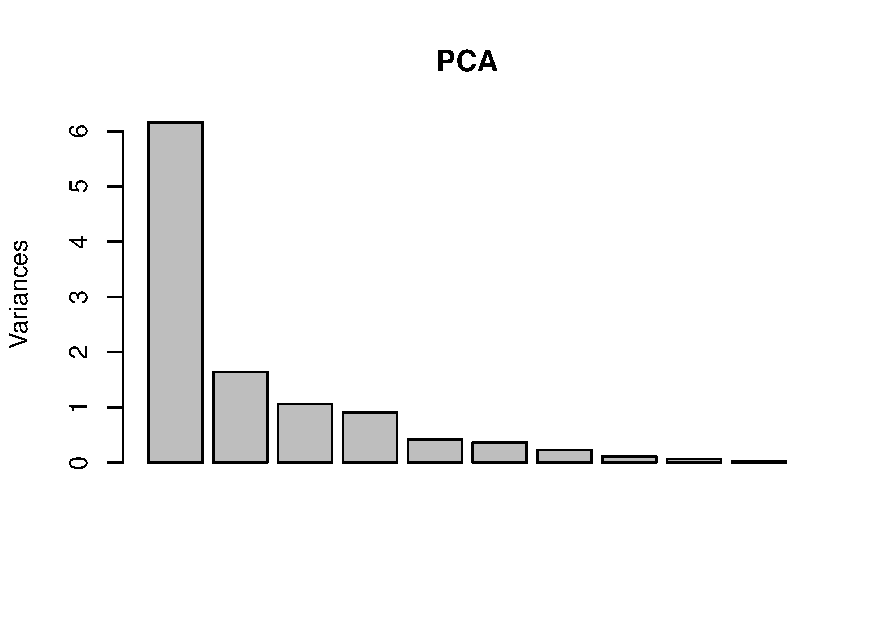
\includegraphics[width=\textwidth]{../code/figures/varianza_total.pdf}
\caption{Varianza total o valores propios de los componentes}
\label{fig:varianza_total}
\end{figure} 


El proceso es el siguiente, se desea obtener las componentes principales $Y$ o combinaciones lineales de coeficientes $A_{11x11}$ de las variables originales $Z$ tal que $Y = ZA$ con $Y_{34x11}$ (componentes principales) y $Z_{34x11}$ (variables originales).

Así, por ejemplo, $y_1 = Za_1$ se obtiene de modo que alcanza la mayor varianza posible, es decir

$$ V(Y_1) = \frac{1}{N-1}Y^{'}_1Y_1 =  \frac{1}{N-1}a^{'}_{1}Z^{'}Za_{1} = a^{'}_1Ra_1 = \lambda_1 = 6.12 $$
(Podemos comprobar el autovalor correspondiente a la componente 1 en figura [\ref{fig:varianza_total}] de varianza total explicada). La varianza del conjunto de variables observadas $Z$ proyectada sobre el vector $a_1$ es $\lambda_1 = 6.12 $. La primera componente o combinación lineal, con el mayor valor propio, es la que mejor resume la información contenida en los datos. 

La segunda componente, que debe maximizar la varianza después de la extracción de $Y_1$, se obtendría calculando el vector $a_2$ tal que
$ y_2 = Za_2$ e $Y_2$ está incorrelado con $Y_1$.
$$ V(Y_2) = \frac{1}{N}Y^{'}_2Y_2 = \frac{1}{N}a^{'}_2Z^{'}Za_2 = ^{'}_2Ra_2 = \lambda_2 =1.63 $$ con $a'_2a_2 =1$.

De modo similar, la tercera componente, $Y_3$, presenta varianza igual a $1.063$.

También podemos ver con summary la desviación típica, la varianza explicada y la acumulada por cada componente principal:
\scriptsize \begin{verbatim}
> summary(PCA) 
Importance of components:
                          PC1    PC2     PC3     PC4    PC5     PC6     PC7     PC8     PC9    PC10    PC11
Standard deviation     2.4818 1.2806 1.03112 0.95154 0.6448 0.60272 0.48187 0.33542 0.24916 0.16420 0.13908
Proportion of Variance 0.5599 0.1491 0.09665 0.08231 0.0378 0.03302 0.02111 0.01023 0.00564 0.00245 0.00176
Cumulative Proportion  0.5599 0.7090 0.80568 0.88799 0.9258 0.95881 0.97992 0.99015 0.99579 0.99824 1.00000
\end{verbatim}
\normalsize

Podemos visualizar estas cantidades en la figura [\ref{fig:proporcion_varianza}]

\begin{lstlisting}
> # Carga del paquete "ggplot2" 
> library("ggplot2")
> varianza_explicada <- PCA$sdev^2 / sum(PCA$sdev^2)
> ggplot(data = data.frame(varianza_explicada, pc = 1:11),
+        aes(x = pc, y = varianza_explicada, fill=varianza_explicada )) +
+   geom_col(width = 0.3) +
+   scale_y_continuous(limits = c(0,0.6)) + theme_bw() +
+   labs(x = "Componente principal", y= " Proporcion de varianza")
\end{lstlisting}

Cada k-ésimo valor propio o autovalor (k=1, ..,11) se interpreta como la parte de la varianza que el k-ésimo eje principal (o sea, la correspondiente componente principal) explica. Y el cociente $\frac{autovalor}{p}$, como la proporción correspondiente a dicha componente; muestra, en consecuencia, la importancia de esta componente en el conjunto.
En particular, para la primera componente tenemos: $\frac{6,1593}{11} =  0,5599 $(véase \% de la varianza en Varianza total explicada en la figura [\ref{fig:varianza_total}])

\begin{figure}[H]
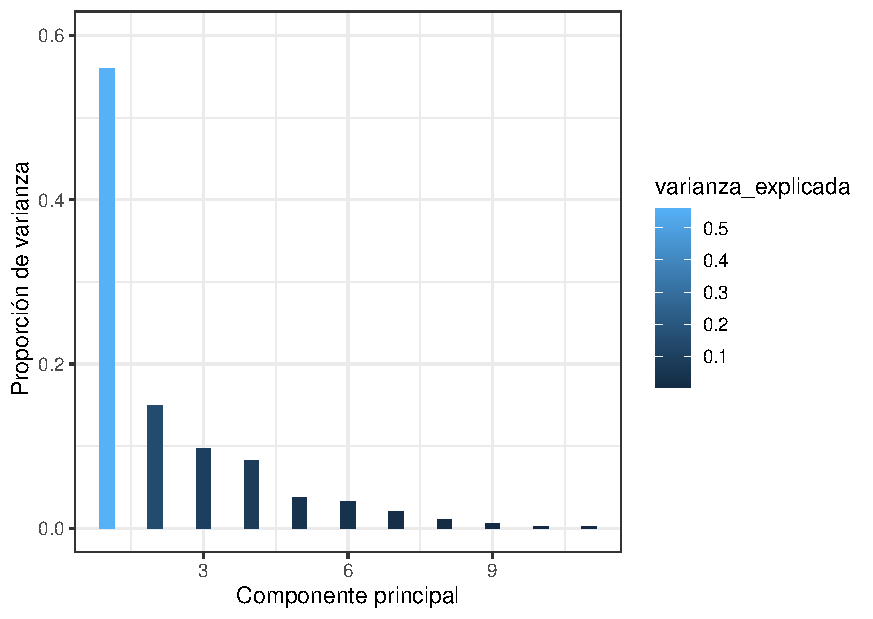
\includegraphics[width=\textwidth]{../code/figures/proporcion_varianza.pdf}
\caption{Proporción de varianza explicada por cada componente principal}
\label{fig:proporcion_varianza}
\end{figure} 

También podemos ver la varianza acumulada por cada componente principal.

\begin{lstlisting}
> varianza_acum<-cumsum(varianza_explicada)
> ggplot( data = data.frame(varianza_acum, pc = 1:11),
+         aes(x = pc, y = varianza_acum ,fill=varianza_acum )) +
+   geom_col(width = 0.5) +
+   scale_y_continuous(limits = c(0,1)) +
+   theme_bw() +
+   labs(x = "Componente principal",
+        y = "Proporcion varianza acumulada")
\end{lstlisting}


\begin{figure}[H]
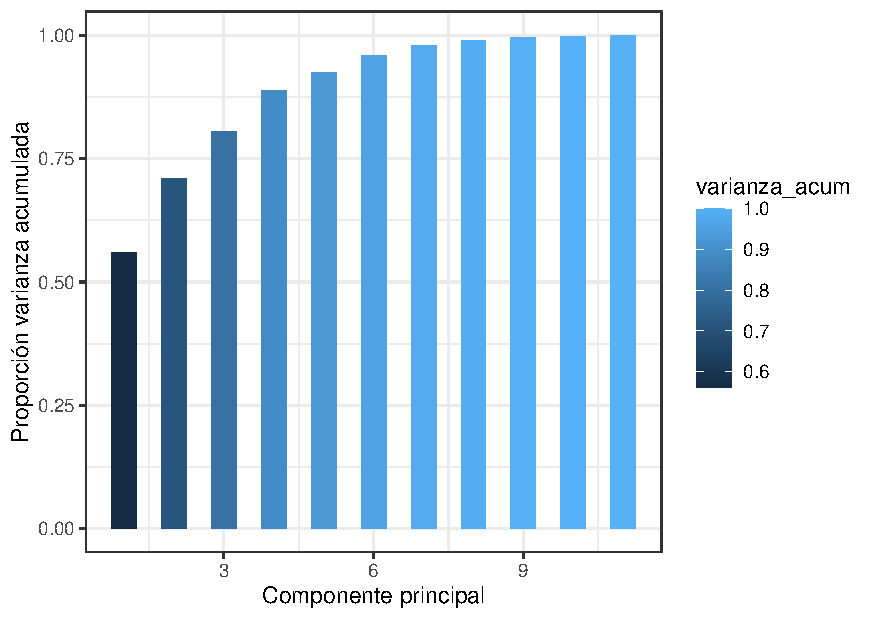
\includegraphics[width=\textwidth]{../code/figures/varianza_acumulada.pdf}
\caption{Proporción de varianza acumulada por cada componente principal}
\label{fig:varianza_acumulada}
\end{figure} 

\section*{Selección número óptimo de componentes principales}
\addcontentsline{toc}{section}{Selección número óptimo de componentes principales}  
Existen diferentes métodos para la selección del número óptimo de componentes principales, en este caso usaremos el explicado en las sesiones tomando las componentes principales cuya varianza sobrepase la media de las varianzas.

\begin{lstlisting}
> PCA$sdev^2
 [1] 6.15934602 1.63988972 1.06319852 0.90543213 0.41577420 0.36326910 0.23219856 0.11250601 0.06208202 0.02696079
[11] 0.01934294
> mean(PCA$sdev^2)
[1] 1
\end{lstlisting}

Vemos que las tres primeras componentes principales es un número óptimo, utilizamos también el método del codo (elbow method) con la varianza acumulada en la figura [\ref{fig:elbow}]

\begin{lstlisting}
> ggplot( data = data.frame(varianza_acum, pc = 1:11),
+         aes(x = pc, y = varianza_acum ,fill=varianza_acum )) + 
+   geom_line(size = 1.5) + 
+   geom_point(size=3, fill="black") +
+   scale_y_continuous(limits = c(0,1)) + 
+   theme_bw() +
+   labs(x = "Componente principal", y = "Proporcion de varianza acumulada")
\end{lstlisting}

\begin{figure}[H]
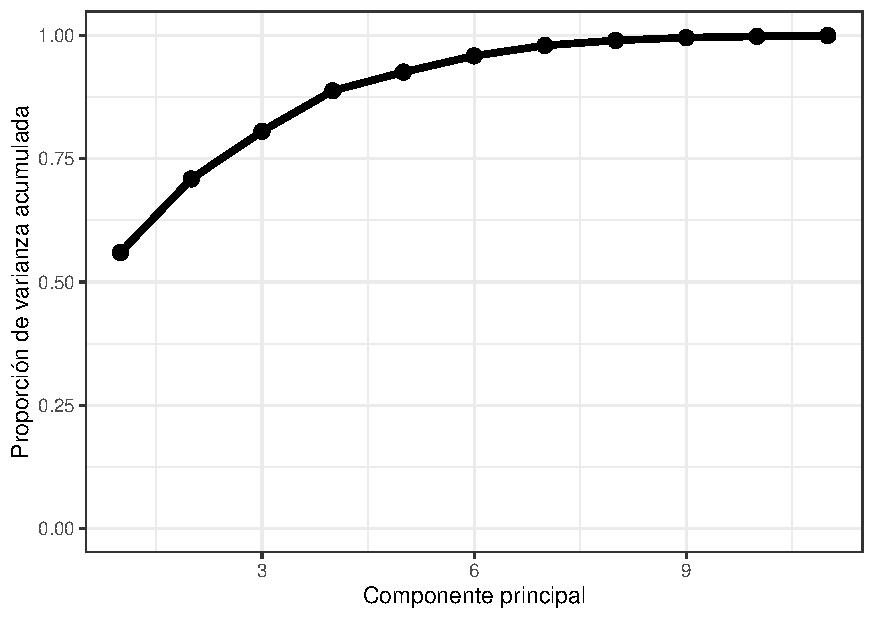
\includegraphics[width=\textwidth]{../code/figures/elbow_method.pdf}
\caption{Método del codo con la varianza acumulada}
\label{fig:elbow}
\end{figure} 

Sólo tres componentes capturan una variabilidad total del 81\% (columna \% acumulado). Esto supone que se puede reducir la dimensionalidad de los datos al pasar de 11 variables observadas a trabajar con sólo 3, sin distorsionar demasiado la información inicial (habrá 19\% de variabilidad en los datos originales del que las tres componentes extraídas no pueden dar cuenta). En sólo 3 dimensiones puede registrarse el 81\% de la variabilidad original, de modo que los tres factores o componentes explican el 81\% de la variabilidad total.

En principio, se prescinde de las componentes asociadas a los valores propios con valores propios inferiores a 1. No obstante, dado que el cuarto valor propio está próximo a 1, quizás estaría bien examinar las posibles ventajas e inconvenientes de su inclusión. Aumentar el número de componentes supone aumentar la dimensionalidad de la información resumida en las componentes aunque no obstante, a veces, un subgrupo de variables importantes podría no quedar bien representado si se omite una componente que recoge la variabilidad del mismo.

\section*{Representación gráfica de los componentes principales}
\addcontentsline{toc}{section}{Representación gráfica de los componentes principales}  

Para realizar representaciones gráficas de los componentes principales, utilizaremos el paquete mostrado en las prácticas \textbf{factoextra} el cuál permite la representación de las componentes principales junto con las variables y observaciones del análisis de componentes principales. Podemos ver la matriz
de coordenadas de las proyecciones de los estados en el subespacio formado por las tres primeras componentes principales
\scriptsize \begin{verbatim}
> t(round(PCA$x[,1:3],3))
    africasu argelia  argentin australi brasil   canada   chile    china    coreasur egipto  
PC1   -1.188   -2.346    1.198    3.207   -0.891    2.757    0.375   -2.175   -0.240   -2.833
PC2   -1.572   -1.881   -1.538   -0.894   -1.347   -1.136   -2.010    2.614    0.226   -0.895
PC3    0.450   -0.811    0.201    0.839    0.899    1.634   -0.302    0.965   -0.022   -1.749
    espa\xf1a   filipina francia  humgria  india    indonesi iran     israel   italia   japon   
PC1       1.977   -2.145    2.641    1.837   -3.767   -3.512   -2.111    2.519    1.879    2.404
PC2      -0.237    0.204   -0.013    1.718    1.259   -0.024   -0.958   -1.133    0.337    0.775
PC3      -1.337    1.274   -0.623   -0.938    1.255    1.264   -0.924   -0.224   -0.086    1.671
    libano   marrueco mejico   nigeria  pakistan polonia  rdaleman reinouni rfaleman rumania 
PC1    0.391   -2.611   -0.429   -4.069   -3.775    1.405    3.001    3.337    3.611    0.707
PC2   -0.939   -0.635   -1.882    0.513   -0.292    1.794    1.804    0.191    0.937    1.725
PC3   -1.808   -0.844    1.061    1.118   -0.456   -0.346   -0.548    0.773   -0.478   -0.577
    turquia  urss     usa      vietnam 
PC1   -2.259    2.066    2.197   -3.157
PC2    1.190    0.852   -0.808    2.056
PC3   -2.393    0.067    0.557    0.435
\end{verbatim}
\normalsize

Mostramos también una matriz de correlaciones cuyos valores representan correlaciones entre cada una de las variables y cada una de las componentes.

\begin{lstlisting}
> cor(datos_pca,predict(PCA)[,1:3])
                 PC1         PC2          PC3
ZPOBDENS  0.16866659  0.49988892  0.078143800
ZTMINFAN -0.93141564 -0.14820207 -0.084681735
ZESPVIDA  0.92237481  0.09310345 -0.004200877
ZPOBURB   0.88870348 -0.37295728 -0.062842442
ZTMEDICO  0.82828728  0.17811944 -0.098854242
ZPAGRICU -0.89903152  0.38341760  0.044837398
ZPSERVI   0.73480310 -0.62593510  0.094693152
ZTLIBROP  0.80892511  0.11387488 -0.072991187
ZTEJERCI  0.05949688  0.22984492 -0.962236433
ZTPOBACT  0.50355447  0.71926891  0.305826185
ZTENERGI  0.82284473  0.25806447 -0.021179701
\end{lstlisting}

Ahora representamos imagenes comparativas entre la primera, segunda y tercera componente. Primera y segunda componente principal en la figura [\ref{fig:primera_segunda}], segunda y tercera en la figura [\ref{fig:segunda_tercera}], y finalmente primera y tercera componentes principales en [\ref{fig:primera_tercera}].

\begin{lstlisting}
> # Esto produce una comparativa entre la primera y segunda componente principal analizando 
> # que variables tienen m?s peso para la definici?n de cada componente principal
> fviz_pca_var(PCA,
+              repel=TRUE,col.var="cos2",
+              legend.title="Distancia")+theme_bw()
> # Esto produce una comparativa entre la primera y tercera componente principal analizando 
> # que variables tienen m?s peso para la definici?n de cada componente principal
> fviz_pca_var(PCA,axes=c(1,3),
+              repel=TRUE,col.var="cos2",
+              legend.title="Distancia")+theme_bw()
> # Esto produce una comparativa entre la segunda y tercera componente principal analizando 
> # que variables tienen m?s peso para la definici?n de cada componente principal
> fviz_pca_var(PCA,axes=c(2,3),
+              repel=TRUE,col.var="cos2",
+              legend.title="Distancia")+theme_bw()
\end{lstlisting}

\begin{figure}[H]
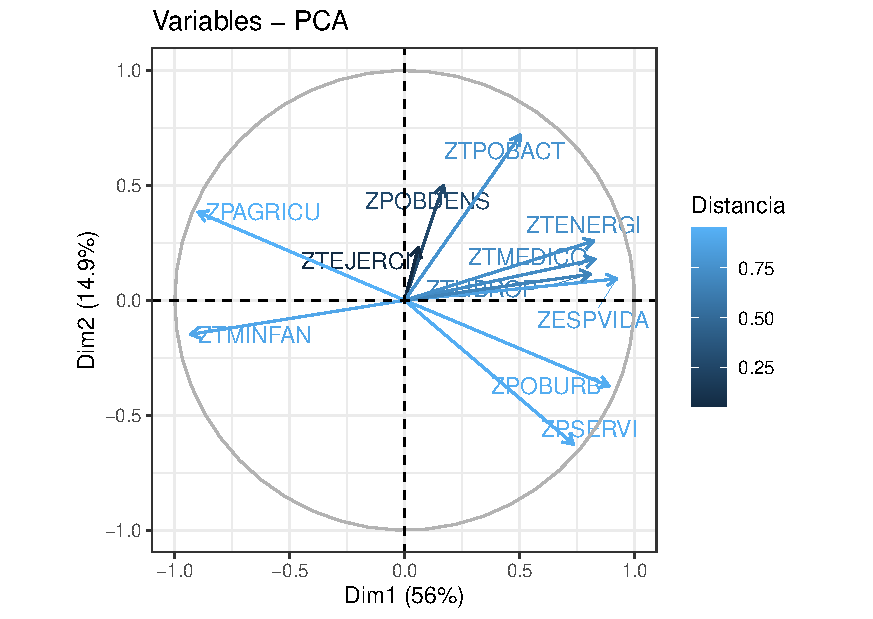
\includegraphics[width=\textwidth]{../code/figures/primera_segunda.pdf}
\caption{Primera y segunda componente principal}
\label{fig:primera_segunda}
\end{figure} 

\begin{figure}[H]
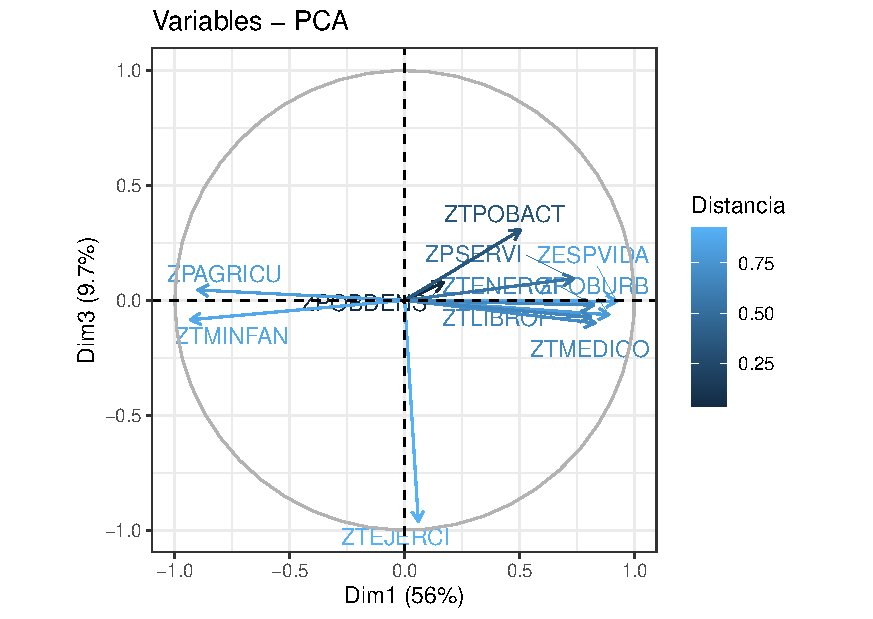
\includegraphics[width=\textwidth]{../code/figures/primera_tercera.pdf}
\caption{Primera y tercera componente principal}
\label{fig:primera_tercera}
\end{figure} 

\begin{figure}[H]
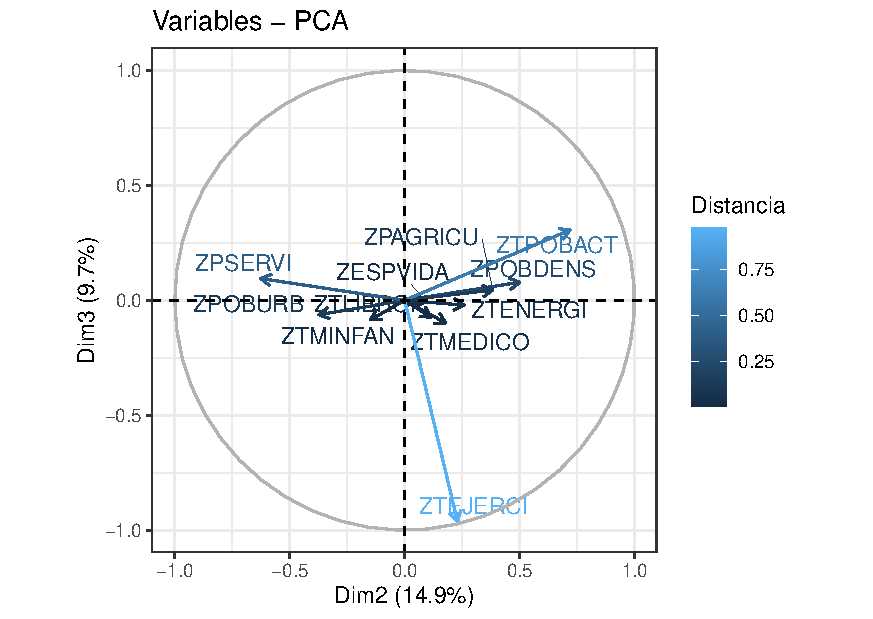
\includegraphics[width=\textwidth]{../code/figures/segunda_tercera.pdf}
\caption{Segunda y tercera componente principal}
\label{fig:segunda_tercera}
\end{figure} 

También es posible representar las observaciones de los objetos junto con las componentes principales mediante la orden \textbf{contrib} de la función \textit{fviz\_pca\_ind}, así como identificar con colores aquellas observaciones que mayor varianza explican de las componentes principales. Repetimos las representaciones anterires mostrando esto

\begin{lstlisting}
> # Observaciones en la primera y segunda componente principal
> fviz_pca_ind(PCA,col.ind = "contrib",
+              gradient.cols = c("#00AFBB", "#E7B800", "#FC4E07"),
+              repel=TRUE,legend.title="Contrib.var")+theme_bw()
> # Observaciones en la primera y tercera componente principal
> fviz_pca_ind(PCA,axes=c(1,3),col.ind = "contrib",
+              gradient.cols = c("#00AFBB", "#E7B800", "#FC4E07"),
+              repel=TRUE,legend.title="Contrib.var")+theme_bw()
> # Observaciones en la segunda y tercera componente principal
> fviz_pca_ind(PCA,axes=c(2,3),col.ind = "contrib",
+              gradient.cols = c("#00AFBB", "#E7B800", "#FC4E07"),
+              repel=TRUE,legend.title="Contrib.var")+theme_bw()
\end{lstlisting}

\begin{figure}[H]
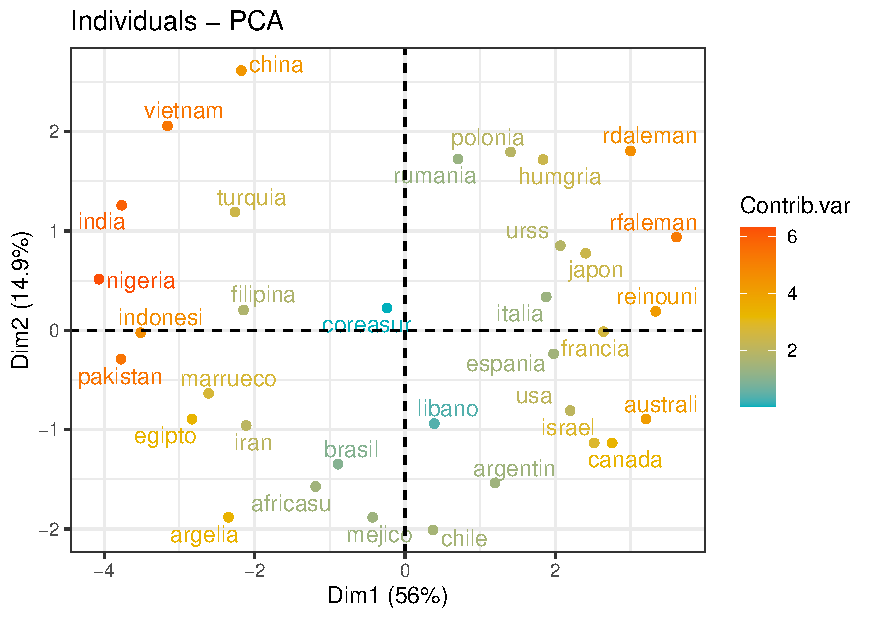
\includegraphics[width=\textwidth]{../code/figures/primera_segunda_obs.pdf}
\caption{Primera y segunda componente principal con observaciones}
\label{fig:primera_segunda_obs}
\end{figure} 

\begin{figure}[H]
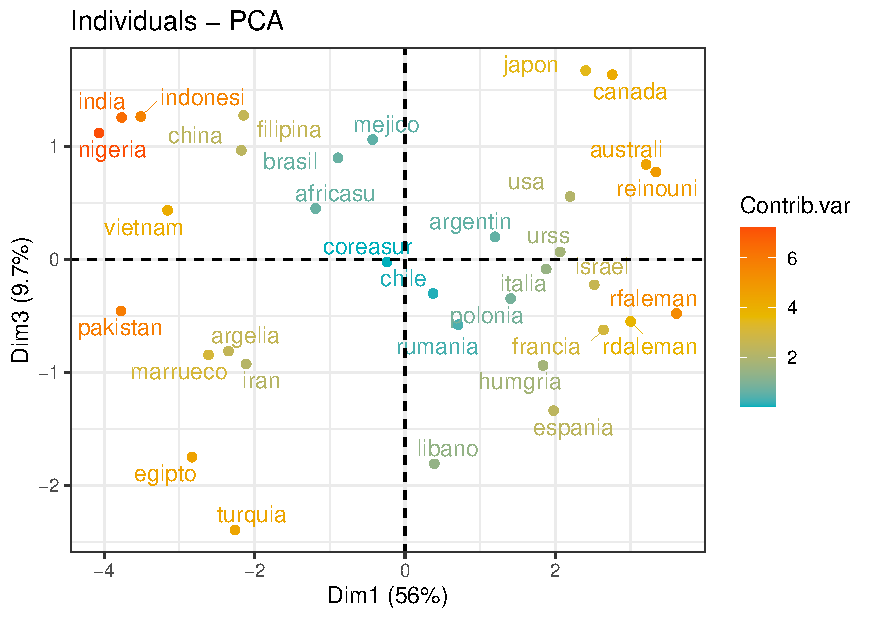
\includegraphics[width=\textwidth]{../code/figures/primera_tercera_obs.pdf}
\caption{Primera y tercera componente principal con observaciones}
\label{fig:primera_tercera_obs}
\end{figure} 

\begin{figure}[H]
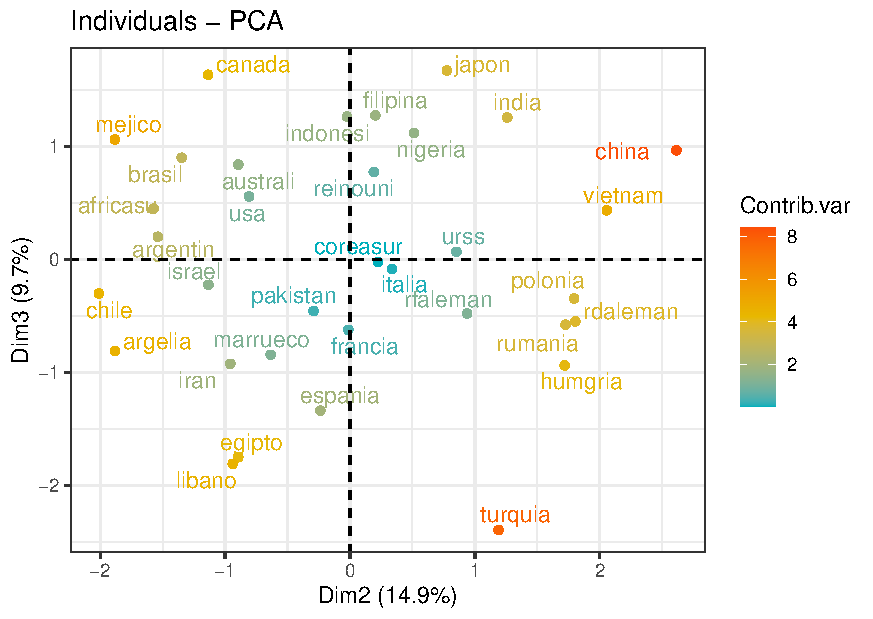
\includegraphics[width=\textwidth]{../code/figures/segunda_tercera_obs.pdf}
\caption{Segunda y tercera componente principal con observaciones}
\label{fig:segunda_tercera_obs}
\end{figure} 

Finalmente podemos realizar una representación conjunta de variables y observaciones que relaciona visualmente las posibles relaciones entre las
observaciones, las contribuciones de los individuos a las varianzas de las componentes y el peso de las variables en cada componentes principal.

\begin{lstlisting}
> # Variables y observaciones en las 1 y 2 componente principal
> fviz_pca(PCA,
+          alpha.ind ="contrib", col.var = "cos2",col.ind="seagreen",
+          gradient.cols = c("#FDF50E", "#FD960E", "#FD1E0E"),
+          repel=TRUE,
+          legend.title="Distancia")+theme_bw()
> # Variables y observaciones en las 1 y 3 componente principal
> fviz_pca(PCA,axes=c(1,3),
+          alpha.ind ="contrib", col.var = "cos2",col.ind="seagreen",
+          gradient.cols = c("#FDF50E", "#FD960E", "#FD1E0E"),
+          repel=TRUE,
+          legend.title="Distancia")+theme_bw()
> # Variables y observaciones en las 2 y 3 componente principal
> fviz_pca(PCA,axes=c(2,3),
+          alpha.ind ="contrib", col.var = "cos2",col.ind="seagreen",
+          gradient.cols = c("#FDF50E", "#FD960E", "#FD1E0E"),
+          repel=TRUE,
+          legend.title="Distancia")+theme_bw()
\end{lstlisting}

\begin{figure}[H]
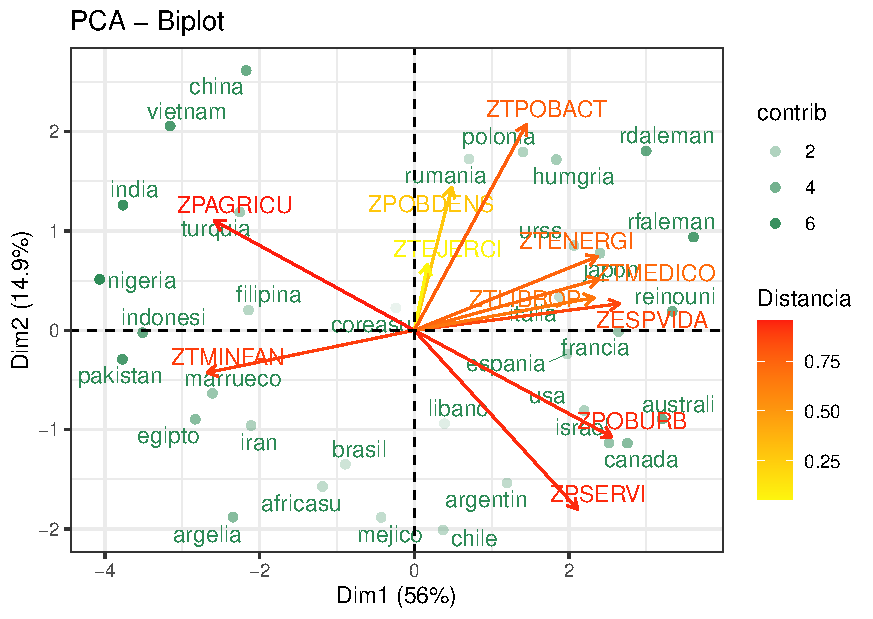
\includegraphics[width=\textwidth]{../code/figures/primera_segunda_todo.pdf}
\caption{Primera y segunda componente principal con todo}
\label{fig:primera_segunda_todo}
\end{figure} 

\begin{figure}[H]
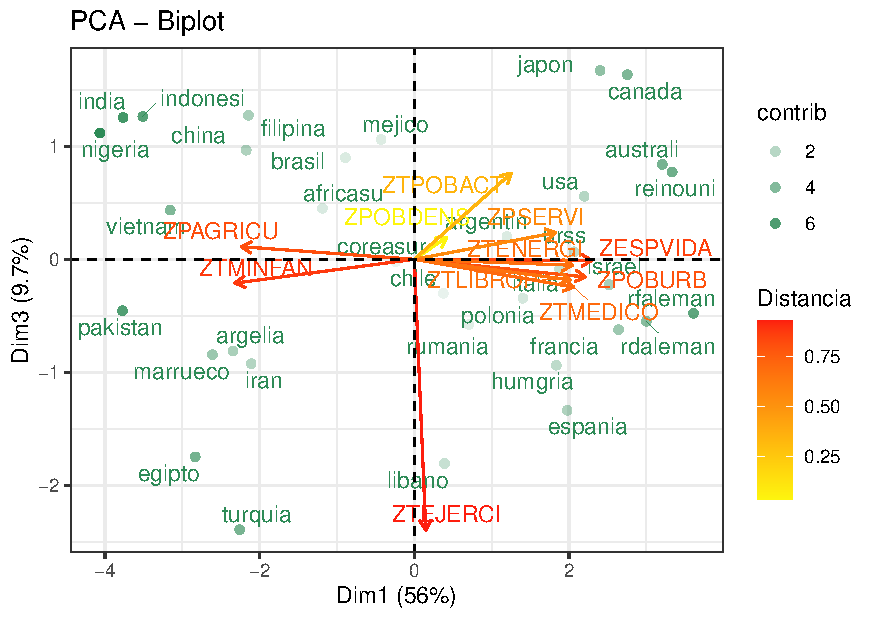
\includegraphics[width=\textwidth]{../code/figures/primera_tercera_todo.pdf}
\caption{Primera y tercera componente principal con todo}
\label{fig:primera_tercera_todo}
\end{figure} 

\begin{figure}[H]
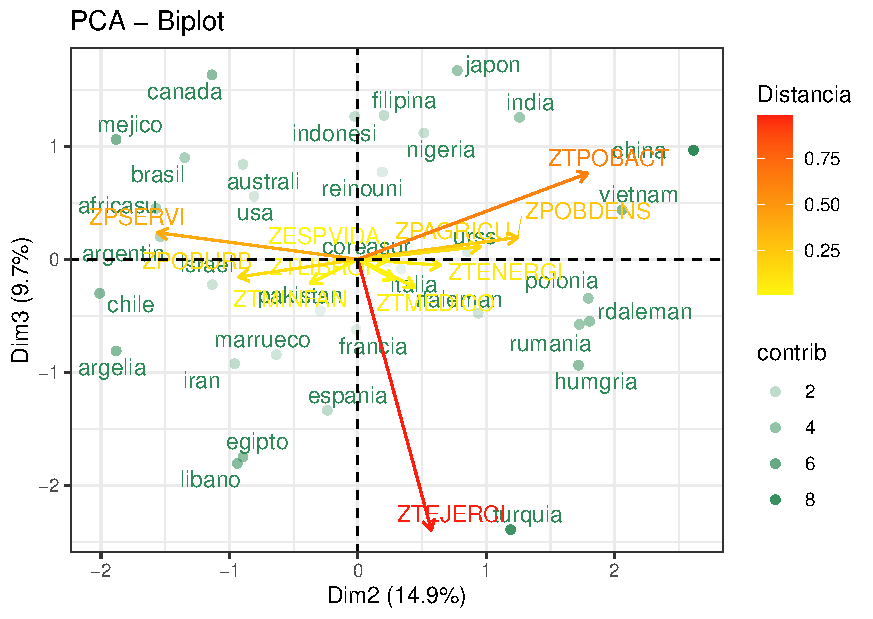
\includegraphics[width=\textwidth]{../code/figures/segunda_tercera_todo.pdf}
\caption{Segunda y tercera componente principal con todo}
\label{fig:segunda_tercera_todo}
\end{figure} 

En la primera componente se ve una comparación de países con fuerte sector de servicios y población urbana frente a países con importante sector agrícola. Países desarrollados vs subdesarrollados diria yo. En la segunda componente destaca la industria y finalmente en la tercera componente densidades de población.

Las variables más correlacionadas con la segunda componente parece que son TPOBACTI, TENERGIA,TMINFAN y TMEDICOS mientras que las variables más importantes para definir la variabilidad registrada en la primera componente son PSERVI, PAGRICUL, POBURB, ESPVIDA, TMINFA. Por otro lado las variables más correlacionadas con la tercera componente son TEJERCIT y POBDENS No estamos ante la situación ideal descrita en párrafos anteriores. 
Algunas variables que presentan presentan correlaciones altas con las componentes 1 y 2 son ESPVIDA, TLIBROPUB, TENERGIA, TMINFAN y TMEDICOS .
Si buscamos caracterizar las componentes según las relaciones observadas con las variables originales es difícil definir una composición específica para las componentes 1 y 2 ya que ambas parecen contraponer los países más desarrollados a los menos desarrollados. Esperanza de vida alta, nivel cultural y bienestar social altos frente a bajos (libros publicados, tasa de médicos por habitantes alta frente a baja, tasa de mortalidad infantil baja frente a alta)

Por último, ya que el objeto de este estudio era reducir la dimensión de las variables utilizadas, es posible obtener las coordenadas de los datos originales tipificados en el nuevo sistema de referencia. De hecho lo tenemos almacenado desde que utilizamos la función \textit{prcomp} para crear la variable PCA. Lo mostramos pequeño por comodidad visual del documento.

\tiny \begin{verbatim}
> head(PCA$x,n=34)
                PC1         PC2         PC3         PC4         PC5         PC6          PC7         PC8         PC9        PC10          PC11
africasu -1.1879510 -1.57174870  0.45044485  0.37814927  1.42283283 -0.27199158 -0.623595597 -0.09144981  0.34753493  0.36296233  0.0009993838
argelia  -2.3462462 -1.88106620 -0.81081919  0.20145035  0.45280276 -0.21767407 -0.113018266  0.67613362  0.31890906 -0.22213535 -0.1452388044
argentin  1.1979236 -1.53833675  0.20077839  0.89727380 -0.38850796 -0.77144470  0.807228821 -0.15129705 -0.40998101  0.13438946 -0.0562911808
australi  3.2068509 -0.89415852  0.83940147  1.06527240  0.55028348  0.38518213 -0.811803953  0.25022260 -0.16193690 -0.38067934  0.2406669888
brasil   -0.8909634 -1.34735175  0.89893299  0.55508246 -0.13891942  0.02175312  0.175309634 -0.23014686 -0.55123723  0.07607427 -0.2189263852
canada    2.7566836 -1.13584507  1.63380445  0.83558450 -0.40111280  1.26624990  0.214600937 -0.41474660  0.39540041 -0.09652726 -0.1070909000
chile     0.3748013 -2.00974285 -0.30168062  0.13027061 -1.15642746 -0.18275397 -0.754674607 -0.13156616 -0.14262580  0.15878588  0.1209991593
china    -2.1745978  2.61356042  0.96542176  0.79447745 -1.51186129  0.21360710 -0.315617302  0.16287419  0.09008596 -0.04968074  0.0175549674
coreasur -0.2395061  0.22577834 -0.02200379 -0.29949146 -0.46326227  1.11284552 -0.035491221  0.39806886 -0.23092496  0.26947888  0.1594077183
egipto   -2.8332447 -0.89472527 -1.74869384 -0.02886629  0.06798311  0.02250445 -0.310866567 -0.08354177 -0.02901969 -0.19432866 -0.0573909279
espania   1.9771834 -0.23696615 -1.33663589  0.04438475 -0.47649830  0.82678614  0.777742199  0.48167714 -0.10099465  0.01181882  0.1049016670
filipina -2.1452831  0.20351988  1.27403374 -0.86565659 -0.56838811 -0.15028934  0.004493093  0.49597736  0.08712967  0.12559592  0.2772966071
francia   2.6414111 -0.01330041 -0.62271201  0.03170101 -0.08010665  0.13854922 -0.260637363  0.10989111  0.31541253 -0.16761311  0.0703157933
humgria   1.8369158  1.71813286 -0.93757556  0.47001001  0.46001652  0.88238111  0.833538559  0.01574888  0.25974597  0.17058796 -0.0509025203
india    -3.7665089  1.25869208  1.25543964 -1.00446829  0.51111537 -0.20212478  0.579046678 -0.03383508 -0.25659043 -0.21257778 -0.1058064933
indonesi -3.5122382 -0.02386264  1.26366487  0.10062250  0.42626703  0.13318440  0.115415733 -0.06815793  0.33036118 -0.08581324  0.0175770992
iran     -2.1106915 -0.95775804 -0.92365774  0.22851570 -0.20529497  0.12404861 -0.318863831  0.50032561 -0.17821369  0.21184100 -0.2075043694
israel    2.5185220 -1.13346621 -0.22444498 -0.43374508 -0.19339430  0.10225569  0.802635989 -0.30878270 -0.14148837 -0.06317868  0.0268765029
italia    1.8793472  0.33682331 -0.08587639 -0.53435523 -0.44626390 -1.29071596  0.829905483  0.37519670  0.17010251 -0.10240096 -0.0920630334
japon     2.4042017  0.77519469  1.67063103 -2.16353425 -0.37124266 -0.68185453 -0.375862213 -0.00357082  0.01804949 -0.07676834 -0.2402706122
libano    0.3908113 -0.93862865 -1.80755715 -2.54094256 -0.39063809 -0.69319566  0.064675345 -0.38259552  0.27888287  0.13462981  0.2033940439
marrueco -2.6111083 -0.63494215 -0.84370677 -0.04560012  0.32314717  0.86093321  0.077375097  0.12651960 -0.09999321 -0.03204079 -0.2011568416
mejico   -0.4292694 -1.88248069  1.06058617  0.18898306 -0.18870059 -0.56822183 -0.038134015  0.30275495 -0.16956075 -0.16756015  0.1298877117
nigeria  -4.0691890  0.51312721  1.11817945  0.17003627  0.74676184  0.22834537  0.182754443 -0.44626412 -0.22970715  0.15560703  0.1771866008
pakistan -3.7752500 -0.29164848 -0.45582169 -0.43747966  0.81514836 -0.13809459  0.282765202 -0.24412230  0.23118350 -0.06426054  0.0721410202
polonia   1.4051850  1.79382646 -0.34557393  0.76060587  0.06958040 -0.49281049 -0.275363943  0.12995559 -0.09238346  0.01584053  0.0187492876
rdaleman  3.0006719  1.80429843 -0.54847315  0.41154507  0.79574301 -0.84486979 -0.720954096 -0.03279271 -0.22607825  0.14754470 -0.0453764779
reinouni  3.3366283  0.19074891  0.77266251 -1.61255080  0.44377012  0.60953258 -0.592216125 -0.31921611 -0.18569892 -0.00228887 -0.0604243295
rfaleman  3.6113690  0.93736385 -0.47800299 -1.52413606  1.06149382  0.72445007  0.104964263  0.11641759 -0.19173155 -0.05768685  0.0292461854
rumania   0.7068599  1.72531630 -0.57683789  0.83431076  0.06419030 -0.20141636 -0.406726190  0.36289963  0.11225930  0.12367151 -0.1884743097
turquia  -2.2589795  1.18954704 -2.39282243  0.64594436 -0.65460455  0.03651040 -0.430409682 -0.82424809 -0.19586549 -0.26359945  0.0158359250
urss      2.0656447  0.85194470  0.06708247  2.12196985  0.75589667 -0.97941596  0.614086633 -0.12622830  0.03093806 -0.01039851  0.1909211317
usa       2.1968825 -0.80816808  0.55718509  0.86676472 -0.76556968 -0.07839738 -0.061084782 -0.51133189  0.47419412  0.12224111 -0.1407301850
vietnam  -3.1568661  2.05632216  0.43464714 -0.24212838 -0.56623978  0.07615199 -0.021218358 -0.10076961  0.13384194  0.02846942  0.0436895774
\end{verbatim}
\normalsize
%% bibliography
\medskip

\printbibliography[
heading=bibintoc,
title={Referencias}
]


\end{document}
